% Código TikZ para tabla de pasos - estilo alternativo
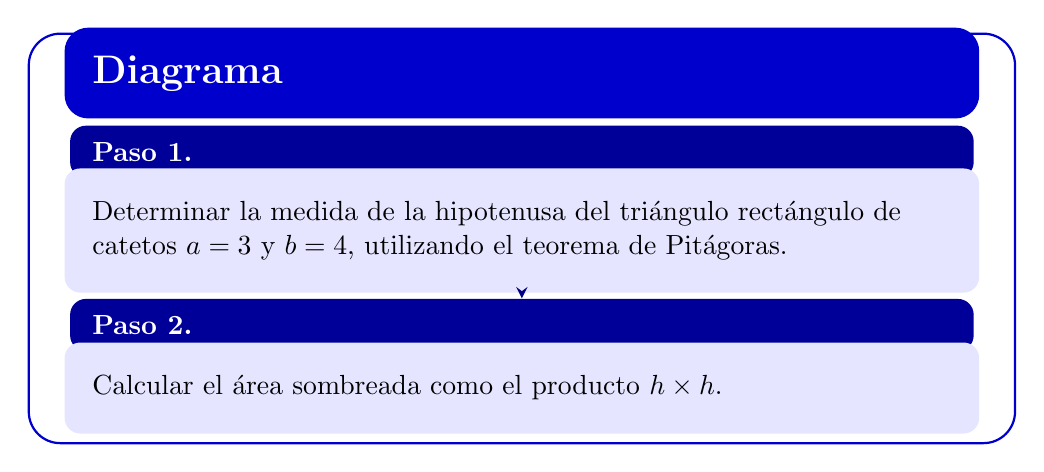
\begin{tikzpicture}[
    box/.style={
        rectangle,
        draw=none,
        text width=0.9\textwidth,
        inner sep=10pt
    },
    step title/.style={
        rectangle,
        draw=none,
        fill=blue!60!black,
        text=white,
        font=\bfseries,
        inner sep=8pt,
        inner ysep=6pt,
        text width=0.9\textwidth,
        rounded corners=2mm
    },
    step content/.style={
        rectangle,
        draw=none,
        fill=blue!10,
        inner sep=10pt,
        inner ysep=12pt,
        text width=0.9\textwidth,
        rounded corners=2mm
    }
]

% Título principal
\node[rectangle, fill=blue!80!black, text=white, font=\Large\bfseries, 
      inner sep=10pt, text width=0.9\textwidth, rounded corners=3mm] 
      at (0,0) {Diagrama};

% Paso 1
\node[step title] (title1) at (0,-1) {Paso 1.};
\node[step content] (content1) at (0,-2) {
    Determinar la medida de la hipotenusa del triángulo rectángulo de catetos $a = 3$ y $b = 4$, utilizando el teorema de Pitágoras.
};

% Paso 2
\node[step title] (title2) at (0,-3.2) {Paso 2.};
\node[step content] (content2) at (0,-4) {
    Calcular el área sombreada como el producto $h \times h$.
};

% Flechas conectoras
\draw[-stealth, thick, blue!50!black] (content1.south) -- (title2.north);

% Borde exterior
\draw[rounded corners=4mm, blue!80!black, thick] 
    (-0.5\textwidth-0.2cm, 0.5cm) rectangle 
    (0.5\textwidth+0.2cm, -4.7cm);

\end{tikzpicture}
